\documentclass[preprint]{aastex}
\usepackage{amsmath}
\usepackage{newtxtext, newtxmath}
\usepackage{booktabs}
\usepackage{graphicx}
\graphicspath{
  {../},
}
\usepackage{minted}

\usepackage{geometry}
\geometry{margin=1in}
\setkeys{Gin}{width=0.6\linewidth, keepaspectratio}  

\usepackage{natbib}
\usepackage{microtype}
\usepackage{xcolor}
\bibliographystyle{apj}

\newcommand\TsqDir{/Users/will/Work/RubinWFC3/Tsquared}
\input{\TsqDir/wfc3-macros.tex}


\begin{document}
\title{Orion fluctuations: New material 2015-10}
\author{W. J. Henney, C. R. O'Dell, G. J. Ferland, M. Peimbert}

\section{Temperature and density diagnostics from the MUSE data}
\label{sec:muse-diagnostic}



\newcommand\DiagFig[3]{\includegraphics{muse-#1-#2-histogram-#3}}

% These 
\newcommand\FourDiagsA[1]{%
  \DiagFig{log10_S_6716_}{log10_N_S_II_}{#1}&
  \DiagFig{log10_S_5518_}{log10_N_Cl_III_}{#1}&
  \DiagFig{log10_S_5755_}{T_N_II}{#1}&
  \DiagFig{log10_S_6312_}{T_S_III}{#1}
}
\newcommand\FourDiagsB[1]{%
  \DiagFig{log10_N_S_II_}{log10_N_Cl_III_}{#1}&
  \DiagFig{T_N_II}{T_S_III}{#1}&
  \DiagFig{log10_N_S_II_}{T_N_II}{#1}&
  \DiagFig{log10_N_Cl_III_}{T_S_III}{#1}
}

\begin{figure}
  \setkeys{Gin}{width=0.2\linewidth}
  \footnotesize
  \begin{tabular}{l cccc}
    Binning & [S II] Density & [Cl III] Density & [N II] Temperature & [S III] Temperature \\
    \raisebox{0.1\linewidth}{\(1 \times 1\)} & \FourDiagsA{full001}\\
    \raisebox{0.1\linewidth}{\(4 \times 4\)} & \FourDiagsA{full004}\\
    \raisebox{0.1\linewidth}{\(16 \times 16\)} & \FourDiagsA{full016}\\
    \raisebox{0.1\linewidth}{\(64 \times 64\)} & \FourDiagsA{full064}\\
  \end{tabular}
  \caption{Derived density and temperature versus surface brightness as a function of
    binning for the full MUSE field}
  \label{fig:muse-dens-temp-diag}
\end{figure}

\begin{figure}
  \setkeys{Gin}{width=0.2\linewidth}
  \footnotesize
  \begin{tabular}{l cccc}
    Binning & [S II] Density & [Cl III] Density & [N II] Temperature & [S III] Temperature \\
    \raisebox{0.1\linewidth}{\(1 \times 1\)} & \FourDiagsA{sweet001}\\
    \raisebox{0.1\linewidth}{\(4 \times 4\)} & \FourDiagsA{sweet004}\\
    \raisebox{0.1\linewidth}{\(16 \times 16\)} & \FourDiagsA{sweet016}\\
    \raisebox{0.1\linewidth}{\(64 \times 64\)} & \FourDiagsA{sweet064}\\
  \end{tabular}
  \caption{Derived density and temperature versus surface brightness as a function of
    binning for the sweet spot}
  \label{fig:muse-dens-temp-diag-sweet}
\end{figure}


\begin{figure}
  \setkeys{Gin}{width=0.2\linewidth}
  \footnotesize
  \begin{tabular}{l cccc}
    Binning & Density--Density & Temperature--Temperature & Density--Temperature & 
    Density--Temperature\\
    \raisebox{0.1\linewidth}{\(1 \times 1\)} & \FourDiagsB{full001}\\
    \raisebox{0.1\linewidth}{\(4 \times 4\)} & \FourDiagsB{full004}\\
    \raisebox{0.1\linewidth}{\(16 \times 16\)} & \FourDiagsB{full016}\\
    \raisebox{0.1\linewidth}{\(64 \times 64\)} & \FourDiagsB{full064}\\
  \end{tabular}
  \caption{Correlations between derived densities and temperatures as a function of
    binning for the full MUSE field}
  \label{fig:muse-dens-temp-correl}
\end{figure}

\begin{figure}
  \setkeys{Gin}{width=0.2\linewidth}
  \footnotesize
  \begin{tabular}{l cccc}
    Binning & Density--Density & Temperature--Temperature & Density--Temperature & 
    Density--Temperature\\
    \raisebox{0.1\linewidth}{\(1 \times 1\)} & \FourDiagsB{sweet001}\\
    \raisebox{0.1\linewidth}{\(4 \times 4\)} & \FourDiagsB{sweet004}\\
    \raisebox{0.1\linewidth}{\(16 \times 16\)} & \FourDiagsB{sweet016}\\
    \raisebox{0.1\linewidth}{\(64 \times 64\)} & \FourDiagsB{sweet064}\\
  \end{tabular}
  \caption{Correlations between derived densities and temperatures as a function of
    binning for the sweet spot.}
  \label{fig:muse-dens-temp-correl-sweet}
\end{figure}



\clearpage

\section{Other half-finished Orion spectra projects}
\label{sec:other}



This is a brain dump of planned and semi-abandoned projects related to
the MUSE, PPAK, and longslit spectra, which are beyond the scope of
the $t^2$ paper. 

\subsection{Balmer and Paschen jump temperatures}
\label{sec:balmer-paschen-jump}

The Balmer jump can be measured from the PPAK spectra.  The Paschen
jump can be measured from the MUSE spectra. 

\begin{figure}
  \includegraphics[width=\textwidth]{\TsqDir/Balmer-Jump}
  \caption{Pilot investigation of Balmer jump from PPAK spectra.}
  \label{fig:balmer-jump-ppak}
\end{figure}

A pilot investigation of the Balmer jump (BJ) is presented in
Figure~\ref{fig:balmer-jump-ppak}.  Spectra are extracted by averaging
over areas ranging in size from 2/9 to 1 square arcminutes (shown by
solid line), with the spectra of individual fibers shown by the cloud
of points.  Each spectrum is shown twice, at two different
magnifications (red and black lines) to emphasize faint and bright
lines.  The location \((x, y)\) in arcsec from \th1{C}, size \((w,
h)\) in arcsec, and number of fibers \(N\) for each region are shown
above each panel.  The intensity of the BJ is estimated manually by
smoothly extrapolating the continuum to either side (\textbf{This is
  not good enough -- see below}) and compared with the intensity of
the H(12--2) Balmer line. 

\paragraph{What we really need to do} is to fit the sum of an atomic
continuum plus a scattered stellar continuum to the observations.  The
atomic continuum (free-bound plus 2-photon) can be modeled with Cloudy
for different temperatures, densities, and this will also give us the
Balmer line spectrum.  The stellar continuum needs to be multiplied by
the effective scattering albedo, which we can assume to be a power law
in wavelength, but the index may vary with position. 

An example is shown in Figure~\ref{fig:balmer-jump-cloudy}, which
shows the stellar spectrum (top) and the H~II region spectrum
(bottom).  There are a few details to iron out:
\begin{enumerate}
\item We need to increase the number of H levels used, so as to get
  more of the higher Balmer lines. \textit{How can Cloudy deal with the
    pseudo-continuum of lines as one approaches the limit without
    using an infinite amount of memory?}
\item The Cloudy reflected spectrum seems to already include a
  dust-scattered stellar component (note the absorption wings visible
  around the H and He emission lines). But we require the atomic
  continuum to be separate from the scattered continuum since they
  need to be varied independently (the size and color index of the
  effective albedo need to be free parameters). \textit{How can we get
  the pure atomic continuum from the Cloudy output? Maybe just turn
  off scattering for the model}
\item Also note that we had to increase the default Cloudy resolution
  to get that nice spectrum.  See
  Appendix~\ref{sec:cloudy-input-script}.  
\end{enumerate}

\begin{figure}
  \includegraphics[width=\textwidth]{\TsqDir/OrionStars/trap-continuum-3500-4020}
  \caption{Cloudy model of the Balmer jump and nearby spectrum.  Blue
    line is the stellar spectrum, which is a composite of Tlusty
    atmosphere models for the Trapezium stars (A, B, C1, C2, and D).
    Green line is the ``Reflected'' continuum diffusely emitted from
    the inner face of the Cloudy model.}
  \label{fig:balmer-jump-cloudy}
\end{figure}


\clearpage
\subsection{Stellar absorption lines in the scattered spectrum}
\label{sec:stell-absorpt-lines}
The figure shows the observed spectra of the Trapezium stars, together
with some comments from 2015-Jan. 

Stellar \ion{O}{2} absorption lines from \th2{A} in the scattered
continuum mean that it is very difficult to detect the \ion{O}{2}
recombination lines on the far side of the Bright Bar. In the Huygens
region, this is not such an issue since there is almost zero
\ion{O}{2} absorption in \th1{C}. 

The \ion{He}{2} 4686 absorption line is very problematic in \th1{C}
because it varies with rotation phase and probably also with viewing
angle, so different parts of the nebula will see different strengths.
However, we can certainly use it in the region around \th2{A}.

\ion{He}{2} 4542 is very strong (depth 0.2) in \th1{C} and seems
constant.  However, we can only use it with the PPAK data since MUSE
does not go that far to the blue.  The same applies to the \ion{Si}{3}
4483 line, which could in principal be diagnostic of the fraction of
scattered light coming from the cooler Trapezium stars \th1{A,B,D}

There is also the \ion{N}{3} 6663 line, which is very strong in some
parts of the nebula (absorption depth of 0.08) but is absent on the
spectra of the brightest OB stars (only seen in \th1{E} and with depth
of only 0.05).  So I have no idea where this is coming from.
\textit{Could there be an hidden luminous cooler giant in Orion~S that
is leaking out light?}

\ion{He}{2} 5411 has some potential, but is contaminated by
[\ion{Fe}{3}] emission. 

\ion{C}{4} 5801.35, 5811.97 are clearly seen in \th1{C} spectrum and
much weaker in \th2{A}, absent in other trapezium stars.
Unfortunately, they are very weak in the nebula. Requires integration over 15x15 arcsec box to have much s/n

Finally, there are the Balmer lines, which show weak underlying
stellar absorption wings. The best ones are H(9--2) 3798 and H(10--2)
3771 because the emission lines are getting weaker to the blue, but the absorption
lines are holding up in strength and the scattered continuum is
getting stronger.  Once you go to higher Balmer lines than that you
run into the [\ion{O}{2}] lines and then they get too close together.
So this is all inaccessible to MUSE, and besides the wavelength
resolution in MUSE is not so good.  But can be done with PPAK and even
better with Adal's longslit spectra.

\begin{figure}
  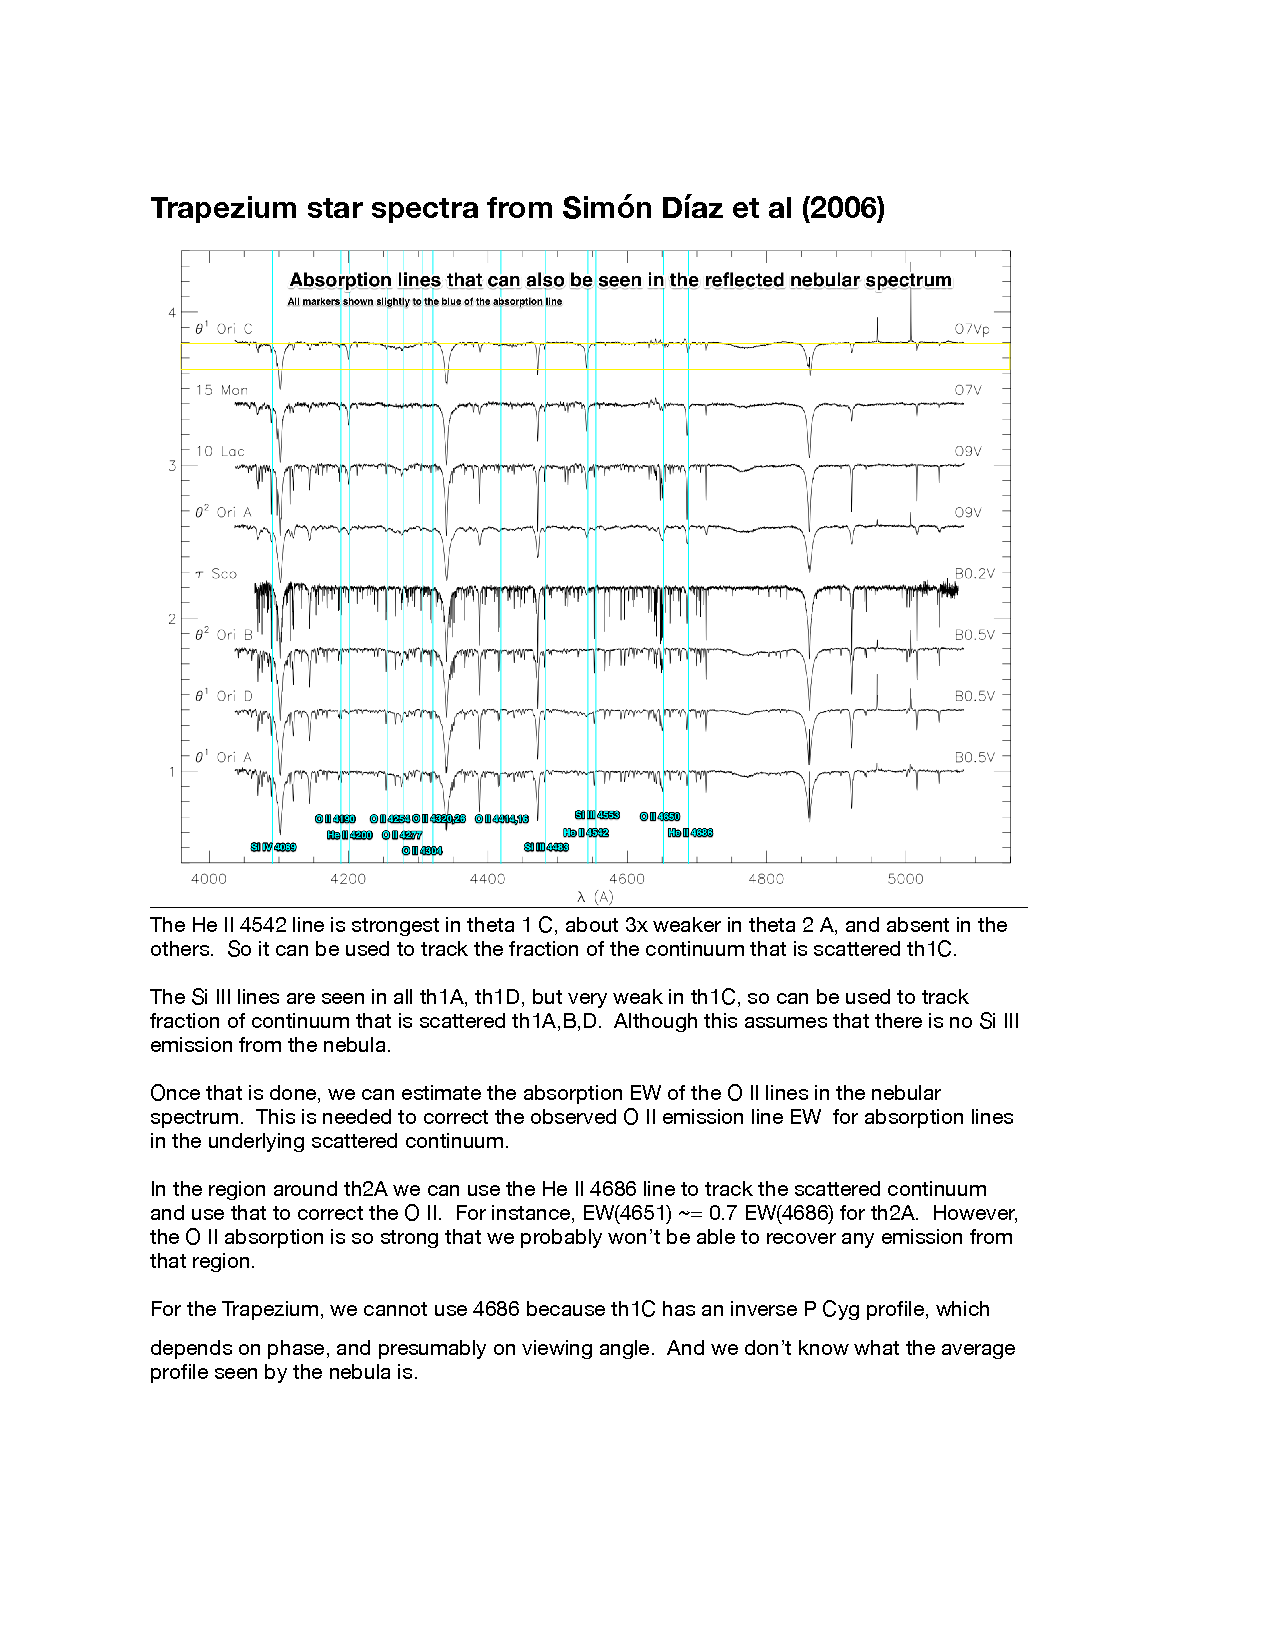
\includegraphics[trim=50 50 50 50, width=\textwidth]{evernote-trap-spectrum}
  \caption{Note from Evernote about scattered absorption lines}
  \label{fig:abs-lines-evernote}
\end{figure}


\subsection{Three different O\(++\) temperatures}
\label{sec:three-different-o++}





\clearpage
\appendix
\section{New calibration of the WFC3 filters with MUSE}
\label{sec:muse-calib}
\citep{Weilbacher:2015a}


\newcommand\calibplot[1]{\includegraphics{wfc3-vs-muse-calib-#1}}

\begin{figure}[p]
  \centering
  \setkeys{Gin}{width=\linewidth}
  \calibplot{F656N}
  \caption[]{Results of spectrophotometric calibration of the WFC3 F656N
    filter.  The vertical axis of the principal plot is the observed
    WFC3 filter count rate after resampling at the \(0.2''\) pixel
    size of the MUSE spectrophotometric observations.  The horizontal
    axis of the principal plot is the predicted count rate calculated
    by folding the MUSE spectrum through the nominal WFC3 filter
    throughput profile.  The grayscale intensity represents the two-dimensional
    histogram over the entire usable WFC3 field of these two
    quantities, weighted by the count rate of each pixel.  The red
    line is the optimum linear fit to the relationship.  The lower
    right inset plot shows the product of the MUSE spectrum (integrated
    over the entire field) and the filter throughput profile.  The
    upper left inset plot shows the distribution of deviations from the
    linear fit for two subsamples of pixels: the red histogram shows
    the subsample with larger than average line/continuum ratio, while
    the blue histogram shows the subsample with smaller than average
    line/continuum ratio.}
\end{figure}

\newcommand\figcontinue[1]{
  \begin{figure}[p]
    \centering
    \setkeys{Gin}{width=\linewidth}
    \calibplot{#1}
    % \addtocounter{figure}{-1}
    \caption{#1}
  \end{figure}
}

\figcontinue{F658N}
\figcontinue{F502N}
\figcontinue{F673N}
\figcontinue{F487N}
\figcontinue{F469N}

\figcontinue{F547M}

\figcontinue{FQ575N}
\figcontinue{FQ672N}
\figcontinue{FQ674N}


\section{Comparison of spectrally derived and filter-derived line
  ratios}
\label{sec:comp-spectr-deriv}

\newcommand\ratioFig[2]{\includegraphics{NebulioMUSE/synthetic#1-vs-true-calib-#2}}

\newcommand\rowOfRatioFigs[1]{
  \ratioFig{-naive}{#1} & \ratioFig{-flat}{#1} & \ratioFig{}{#1} 
}
\begin{figure}
  \setkeys{Gin}{width=0.33\linewidth}
  \centering
  \begin{tabular}{lll}
    \rowOfRatioFigs{4861-6563} \\
    \rowOfRatioFigs{5755-6583} \\
    \rowOfRatioFigs{6716-6731} \\
    \rowOfRatioFigs{6716-6731-N} \\
  \end{tabular}
  \caption{Successive improvements in line ratio estimation using
    synthetic filters with the MUSE dataset}
\end{figure}


\clearpage
\section{Code and input file listings}

\subsection{Cloudy input script for
  Figure~\ref{fig:balmer-jump-cloudy}}
\label{sec:cloudy-input-script}
Based on an earlier script of Gary's from the [\ion{N}{1}] project,
but stops at i-front, since we are not interested in the PDR

\inputminted[fontsize=\footnotesize]{text}{\TsqDir/OrionStars/trap.in}

Note that the figure was produced with a custom continuum, which is
much finer around the Balmer jump wavelength.  This requires editing
the file \verb|continuum_mesh.ini| in the Cloudy source tree.  The
edited version is as follows:

\inputminted[fontsize=\footnotesize]{C}{/Users/will/Work/CLOUDY/git-svn/data/continuum_mesh_balmer_jump.ini}

\subsection{Tables and scripts for MUSE reduction and analysis}
\label{sec:MUSE-tabs-scripts}

\paragraph{\texttt{wavsec-startwavs.tab}: starting wavelength of each
  section that the full cube is split into}
\inputminted[fontsize=\footnotesize,obeytabs,tabsize=12]{text}{wavsec-startwavs.tab}

\paragraph{List of lines that we try and extract from the MUSE datacube}
\inputminted[fontsize=\footnotesize,obeytabs,tabsize=12]{text}{basic-line-list.tab}

\paragraph{\texttt{extract-em-line.py}: extract emission lines from cube}
\inputminted[fontsize=\footnotesize]{python}{extract-em-line.py}

\paragraph{\texttt{plot-em-line-spec.py}: plots average spectrum for
  each line}
\inputminted[fontsize=\footnotesize]{python}{plot-em-line-spec.py}

\paragraph{\texttt{multibin-map.py}: Rebin the MUSE line maps at
  multiple resolutions}

\inputminted[fontsize=\footnotesize]{python}{multibin-map.py}

Run the above script on all extracted lines:
\begin{minted}[fontsize=\footnotesize]{sh}
linelist=LineMaps/linesum-*[0-9][0-9][0-9][0-9].fits
for line in $linelist; do
    echo "Processing $line"
    time python multibin-map.py $line > ${line}-multibin.log
done
\end{minted}

\bibliography{BibdeskLibrary-slavoj}


\end{document}
%%% Local Variables:
%%% mode: latex
%%% TeX-master: t
%%% End:


